\chapter{WebSocket Application Deployment}
\label{chapter:webSocketApplicationDeployment}

This chapter introduces various considerations when deploying WebSocket applications and talks about containerized deployment and other deployment considerations..

\section{WebSocket Connection Types}

When deploying a WebSocket application there are requirements that need to be taken into account. These requirements depend on the nature of the deployed applications and the traffic handled by their runtime environments. In addition, devices like reverse proxy servers, firewalls and load-balancing routers must be taken into account when designing and implementing systems that utilize the WebSocket protocol. A large proportion of the internet infrastructure is predominantly configured for HTTP traffic and not familiar with the WebSocket protocol. This can introduce various challenges when deploying applications that utilize.

\subsection{Unencrypted WebSocket Traffic}

The deciding factor whether a client and a server successfully manage to establish an unencrypted WebSocket connection (\texttt{ws://} on port 80) in production environments is usually interaction with proxy servers located on the communication path. Connections through an explicit proxy servers, that a client is explicitly configured to use, will most likely lead to a successful connection upgrade during the WebSocket handshake as they are configured to allow the \texttt{CONNECT} method. When WebSocket traffic flows through transparent proxies it is likely to be dropped as the proxy will likely remove certain header information, like the connection header, which will lead to a failed WebSocket handshake. Even though a transparent proxy server is not configured to remove the connection header the WebSocket connection is still unlikely to succeed as it behaves differently than HTTP traffic which is what the server has been configured for. This will likely be the case until the infrastructure of the internet will more frequently be configured to handle traffic long lived connections of protocols like WebSocket and HTTP/2. Figure x shows interaction between WebSocket and different types of proxy servers and whether a successful connection establishment is likely.
\\
\begin{figure}[h!]
	\centering
	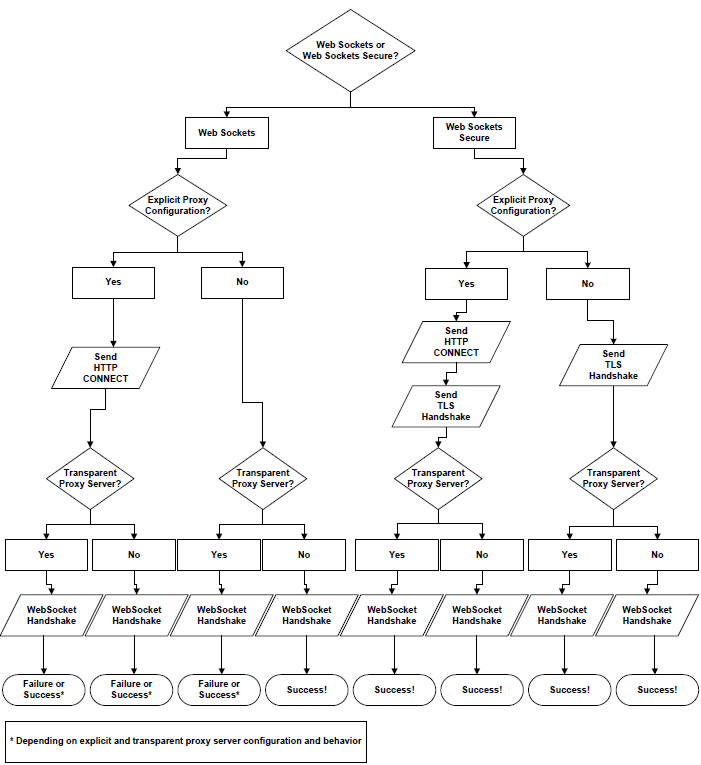
\includegraphics[width=0.9\textwidth]{images/websocketProxyServer}
	\caption{Interaction between WebSocket applications and proxy servers \cite{wang2013definitive}}
	\label{fig:webSocketMessagingSystem}
\end{figure}

\newpage
\subsection{Encrypted WebSocket traffic}

Encrypted WebSocket traffic (\texttt{wss://} on port 443) is more predictable than unencrypted traffic since it is less dependent on the intermediaries on the connection path. In the case of explicit proxies a TLS handshake takes place after a successful WebSocket connection upgrade handshake. Afterwards an encrypted and unhampered WebSocket communication channel is established between a client and a server. When a WebSocket connection is established in the presence of transparent proxies a successful handshake is considerably more likely as the communication is encrypted and proxies are generally configured to accept that kind of traffic. TLS encrypted traffic leads to slightly increased CPU consumption on both sides of the communication but its benefits significantly outweigh that drawback.

\subsection{Fallback Strategies and WebSocket Abstractions}

In addition to the possible issues proxy servers and other intermediaries can cause for WebSocket traffic some older browsers lack support for the protocol. Currently, all modern browsers\footnote{\url{http://caniuse.com/websocket}} support the protocol but WebSocket applications that are intended for widespread use and corporate environments, where older browsers might be common, should have a decent fallback strategy. Because of the uncertainty in the environment where WebSocket applications can be deployed polyfills, which are libraries that implement a standard API using legacy browser features, can be a good solution. In the case of WebSocket a polyfill library would use HTTP-based communication patterns like polling or long-polling as fallback options. Another option would be to use a plugin, like Adobe Flash, capable of establishing a full-duplex communication channel with TCP sockets. That option use usually the least favorable one as it requires the user to explicitly install the plugin which can lead to a bad user experience.
\\ \\
Engine.io\footnote{\url{https://github.com/Automattic/engine.io}} is a Node.js WebSocket implementation that adds increased reliability when establishing a WebSocket connection between a client and a server. The most important design decision of Engine.io is that communication is initiated with a long-polling connection that is upgraded to better transports that are tested during the first moments of the connection establishment. This approach to WebSocket connection establishment is based on empirical experience working with the protocol in production environments in the vicinity of proxies and other network intermediaries. Experiments even seem to indicate that a WebSocket abstraction like Engine.io can increase data throughput without a significant impact on permornace \cite{ozger2014websocket}. There exists numerous other WebSocket implementations and frameworks that add different levels of abstractions and connection management. These extensions seem to be necessary to increase the reliability of unencrypted WebSocket traffic while the majority of the underlying infrastructure of the web is predominantly configure for HTTP traffic.

\subsection{WebSocket Connection Establishment Analysis}

For the analysis of WebSocket connection establishment, network traffic of an echo server for unencrypted, encrypted and abstracted WebSocket traffic was recorded. The purpose of the analysis is to better understand how the WebSocket protocol will behave in a production environment and evaluate how reliable WebSocket-based communication can be implemented.
\\ \\
The data in the analysis was generated through periodic data transfer of text and binary data following the different WebSocket connection establishments. The network traffic was captured with the \texttt{tcpdump} Unix tool and the data was presented with Wireshark\footnote{\url{https://www.wireshark.org/}}, the package analysis tool.
\\
\begin{figure}[h!]
	\centering
	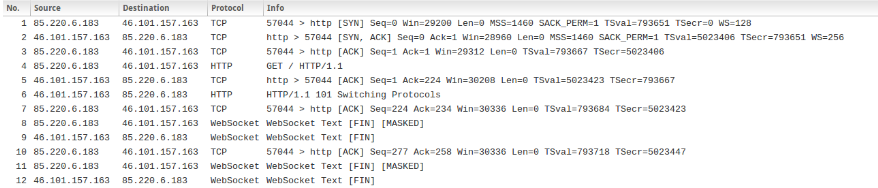
\includegraphics[width=1\textwidth]{images/ws_dump}
	\caption{Network traffic for a \texttt{ws://} connection establishment}
	\label{fig:wsTraffic}
\end{figure}

\noindent
The interesting parts of figure~\ref{fig:wsTraffic} are package No. 4, where the client requests a connection upgrade, and package No. 6 where the server inform the client of a protocol switch to upgrade the connection from HTTP to WebSocket. After the connection establishment data flows between the client and server using the WebSocket protocol. This kind of network traffic would be filtered in many network environments because of its difference from standard HTTP traffic.
\\
\begin{figure}[h!]
	\centering
	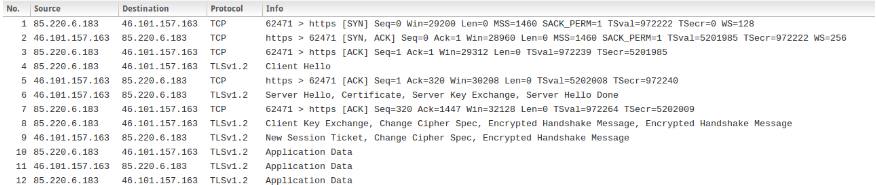
\includegraphics[width=1\textwidth]{images/wss_dump}
	\caption{Network traffic for a \texttt{wss://} connection establishment}
	\label{fig:wssTraffic}
\end{figure}

\noindent
Connection establishment using \texttt{wss://} is largely hidden from network tools like can be seen in figure~\ref{fig:wssTraffic}. This is the reason WebSocket traffic over TLS is more likely to succeed than unencrypted WebSocket traffic. Package No. 4 shows the beginning of the TLS handshake, package No. 6 shows the certificate exchange and package No. 8 shows the key exchange. Afterwards, the application data is encrypted and network intermediaries treat it like regular HTTPS traffic which makes WebSocket and other types of long-lived connections possible.
\\ \\
Figure~\ref{fig:engineioTraffic} shows the process of establishing a bidirectional communication channel with Engine.io which in this case results in a WebSocket connection. The main goals of Engine.io are to provide good server performance and user experience across all browsers given the most suitable technologies available. The case is that traditional HTTP mechanisms are often capable of providing similarly good user experience such as more sophisticated technologies. The client makes the initial upgrade request to switch to a WebSocket connection in package No. 23. Before that the client makes two poll requests in packages No. 4 and 18. Even after the update requests has been made and the server is in the process of of upgrading the request the client makes two more poll requests in packages No. 27 and 43. From package No. 57 and onward a WebSocket connection has been fully established which is at that point considered to be the best mode of communication by Engine.io so it replaces the long-polling. This whole process takes place with out the knowledge of most users and leads to a superior user experience and network utilization than approaches that are fully WebSocket-based or use some form of polling. This procedure is the best approach to establishing an unencrypted WebSocket connection in accordance with the infrastructure of the web based on the experience of the Engine.io developers.

\newpage
\begin{figure}[h!]
	\centering
	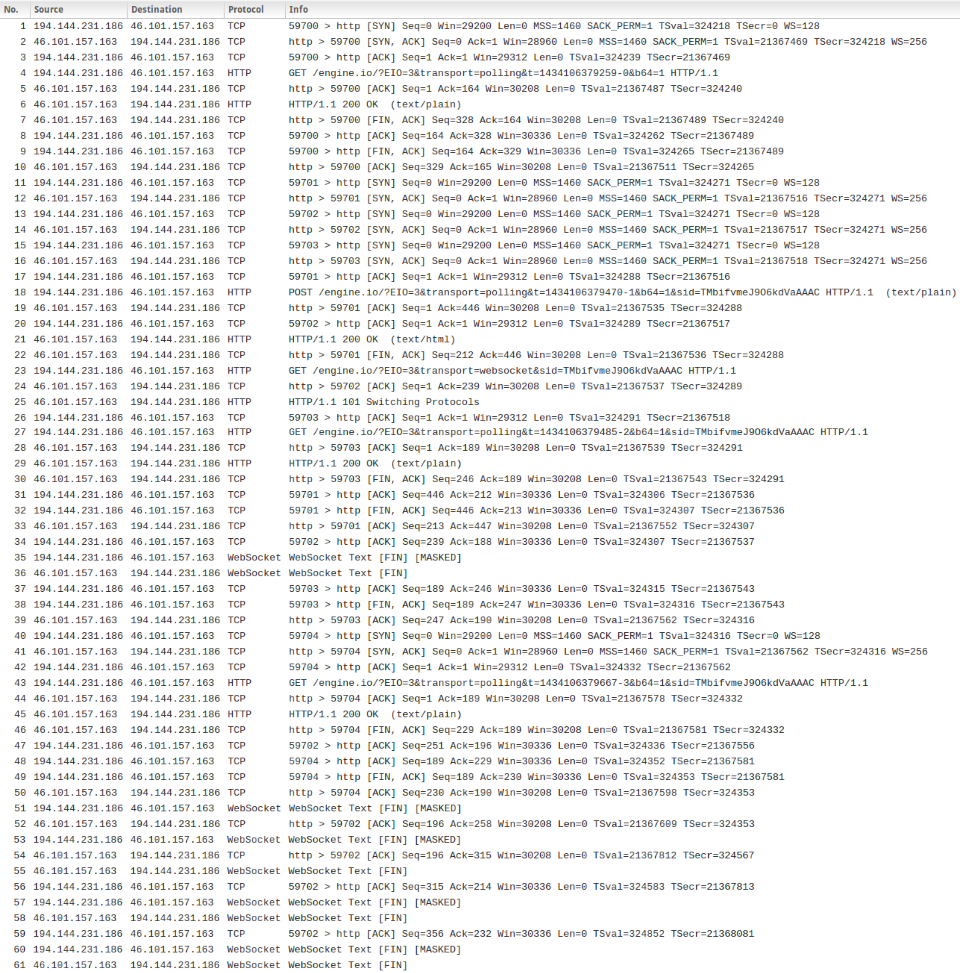
\includegraphics[width=1\textwidth]{images/engineio_dump}
	\caption{Network traffic for an abstracted \texttt{ws://} connection establishment using Engine.io}
	\label{fig:engineioTraffic}
\end{figure}

\section{Containerized WebSocket Infrastructure}

Something general about Docker..

\subsection{Deploying Containers}

\begin{itemize}
\item How to deploy
\item How to manage (continuous integration something..)
\item How are Netflix, Spotify etc. using Docker in production..
\item name drop some common tools: docker-compose, ...
\item A couple of Dockerfile files in the appendix
\item talk about linking containers (as can be seen in the setup of monitoring in the next chapter)
\end{itemize}

\subsection{Monitoring Containers}

\begin{itemize}
\item Why is it important to monitor
\item how to set up monitoring with cAdvisor, influxdb and Grafana..
\end{itemize}

\section{Other Deployment Considerations}

In addition to deciding a suitable communication strategy there are other factors that must be taken into consideration when deploying WebSocket applications. Network intermediaries that can impact deployed services are either located on the path between its users and the internet or between its servers and the internet. Most often it is impossible to influence the configuration of the users network and proxies on external networks so communication strategies like the ones that have been mentioned before must be utilized. As the adoption of HTTP/2 increases networks will more commonly be configured to allow long-lived connection which will increase the effectiveness of the WebSocket protocol. Infrastructure on the serving path that can be configured and is intended for WebSocket traffic should be tuned for long-lived connections. That is something that takes special care as most network infrastructure is configured by default for short lived HTTP traffic. Nginx for example is configured to timeout connections that have been idle for 60 seconds unless the timeout interval is specially increase like can be seen in the configuration file in Appendix~\ref{chapter:chapter:appendix-reverseProxy}. The number of expected concurrent connections must also be taken into account as most Unix systems have a pre-configured limit on the number of open sockets. This limit can be seen with the \texttt{ulimit -a} command and is usually set at 1024. To increase the limit the \texttt{-n} flag can be used (\texttt{ulimit -n 2048} to double the default limit of allowed concurrent sockets). Other areas of consideration include identifying critical areas more monitoring, introducing ping intervals to prevent connection timeouts and identifying where throttling might improve performance. WebSocket-based applications introduce a range of operational challenges not associated with HTTP-based applications that must be dealt with accordingly if the benefits of the protocol are to be fully reaped.

\begin{itemize}
\item Browser support?!
\item protocol extensions

\end{itemize}